% =====================================================================
% Journal of Computer Science and Technology (JCST) submission
%
% Springer / Institute of Computing Technology, CAS / China Computer
% Federation.  Scopus and SCI indexed.  Subscription journal: no article
% processing charge unless you elect open access.
%
% ---------------------------------------------------------------------
% READ THIS FIRST
% ---------------------------------------------------------------------
% JCST mandates its own LaTeX class, distributed only from the journal's
% download page:
%
%     https://jcst.ict.ac.cn/  ->  "Download Templates"  ->  JCST Submit
%     Template (LaTeX).  The package also contains JCST.bst.
%
% That class file is NOT redistributable and is not in any TeX bundle, so
% this file cannot use it directly.  What this file does instead:
%
%   * Everything between BODY-BEGIN and BODY-END conforms to JCST's
%     published Instructions for Authors and is written to be pasted into
%     the official Submit Template with no edits.
%   * The preamble below EMULATES the JCST page layout so the manuscript
%     compiles and can be proof-read now.  It is scaffolding, not the
%     journal's class.  Discard it when you move the body across.
%
% TO PRODUCE THE REAL SUBMISSION
%   1. Download the JCST Submit Template (LaTeX).
%   2. Open its main .tex file.
%   3. Copy everything between BODY-BEGIN and BODY-END into it.
%   4. Point \bibliographystyle at JCST.bst, or keep the inline
%      thebibliography block below, which already matches JCST's format.
%   5. Compile and confirm the page count lands in 8-16 pages.
%
% ---------------------------------------------------------------------
% JCST REQUIREMENTS THIS FILE SATISFIES
% ---------------------------------------------------------------------
%   Abstract         100-250 words, no undefined abbreviations, no
%                    mathematical expressions, no bibliographic
%                    references.                         -> 243 words
%   Keywords         3-5, alphabetical order, comma separated.  -> 5
%   Length           Research Paper: 8-16 pages including text, figures,
%                    tables and references.
%   Review           DOUBLE-BLIND.  No author name, affiliation,
%                    acknowledgement or identifying repository URL
%                    appears anywhere below.
%   Tables           Vertical three-line only; caption above in Title
%                    Case; notes beneath introduced by "Note:".
%   Figures          Cited as Fig.1, Fig.2 (no space); caption below
%                    beginning "Fig.N.".
%   Citations        Numbers in square brackets, numbered in order of
%                    first citation.
%   Biography        Supplied only on acceptance, so omitted here.
%   Running head     Shortened title within 45 characters.
% =====================================================================

% --------------------------- EMULATION PREAMBLE ----------------------
% Replace wholesale with the official JCST template.
\documentclass[9pt,twocolumn]{extarticle}

\usepackage[letterpaper,top=0.9in,bottom=0.9in,left=0.72in,right=0.72in,
            columnsep=0.26in]{geometry}
\usepackage{amsmath}
\usepackage{newtxtext}
\usepackage{newtxmath}
\usepackage{graphicx}
\usepackage{booktabs}
\usepackage{caption}
\usepackage{array}
\usepackage{url}
\usepackage[hidelinks]{hyperref}
\usepackage{xcolor}
\usepackage{titlesec}
\usepackage{fancyhdr}
\usepackage{balance}
\usepackage{changepage}   % adjustwidth, for the indented abstract block

\graphicspath{{figures/}}

% JCST caption style: figures "Fig.1." below; tables "Table 1." above.
\captionsetup[figure]{labelsep=period,labelfont=bf,font=small,
                      name=Fig.,skip=4pt}
\captionsetup[table]{labelsep=period,labelfont=bf,font=small,
                     justification=centering,skip=4pt}
\renewcommand{\thefigure}{\arabic{figure}}
\newcommand{\figref}[1]{Fig.\ref{#1}}
\newcommand{\tabref}[1]{Table~\ref{#1}}
% Table notes, per JCST: beneath the table body, introduced by "Note:".
\newcommand{\tabnote}[1]{\par\vspace{2pt}\footnotesize\textit{Note:} #1}

\titleformat{\section}{\centering\normalsize\bfseries}{\thesection}{0.6em}{}
\titleformat{\subsection}{\normalsize\bfseries}{\thesubsection}{0.6em}{}
\titlespacing{\section}{0pt}{8pt}{5pt}
\titlespacing{\subsection}{0pt}{7pt}{3pt}

\pagestyle{fancy}
\fancyhf{}
% JCST: shortened title within 45 characters. This is 43.
\fancyhead[L]{\footnotesize Deterministic Guardrails and Judge Variance}
\fancyhead[R]{\footnotesize\thepage}
\renewcommand{\headrulewidth}{0pt}

% Flags an item the author must supply before submitting.
\newcommand{\REPLACE}[1]{\textcolor{red}{\textbf{[REPLACE: #1]}}}

\setlength{\parindent}{1.2em}
\setlength{\abovedisplayskip}{4pt}
\setlength{\belowdisplayskip}{4pt}
% ------------------------- END EMULATION PREAMBLE --------------------

\begin{document}

% ---------------------------------------------------------------------
% CAMERA-READY AUTHOR BLOCK -- KEEP COMMENTED OUT FOR SUBMISSION
%
% JCST reviews double-blind, so none of this may appear in the file the
% reviewers read. Author details go on the separate title page
% (title_page.tex) and into the submission system instead.
%
% Uncomment this and delete the "Anonymous Submission" lines below ONLY
% when preparing the camera-ready version after acceptance.
%
% \begin{center}
%   {\normalsize
%    Rishav Gupta\quad Prachi Sharma\quad Danish Kaul\quad
%    Dishant Sherawat\par}
%   \vspace{3pt}
%   {\footnotesize School of Engineering and Technology,
%    Sushant University, Gurugram, Haryana, India\par}
%   {\footnotesize E-mail: \{...\}@sushantuniversity.edu.in\par}
% \end{center}
% ---------------------------------------------------------------------

% ============================== BODY-BEGIN ==========================
% Paste everything from here to BODY-END into the official JCST
% Submit Template.  Nothing below depends on the emulation preamble
% except \figref, \tabref and \tabnote, which are one-line macros
% defined above and can be inlined if the template objects.

\twocolumn[
  \begin{@twocolumnfalse}
  \begin{center}
    {\large\bfseries Deterministic Guardrails and Variance-Aware
     Evaluation for Multi-Agent Content Personalization\par}
    \vspace{6pt}
    {\normalsize\itshape Anonymous Submission\par}
    \vspace{2pt}
    {\footnotesize Author and affiliation details are withheld in
     accordance with JCST's double-blind review process.\par}
  \end{center}
  \vspace{10pt}

  \begin{adjustwidth}{0.5cm}{0.5cm}
  \noindent\textbf{Abstract}\quad
  Large language models produce fluent marketing text, yet they routinely
  fabricate quantitative claims and drift outside the task they were asked to
  perform, and the field lacks settled practice for deciding whether an
  engineering fix has genuinely helped. This paper reports a system together
  with a measurement study. The system is a personalized content generator in
  which five narrow agents share a three-level user profile, and in which two
  interventions are deliberately deterministic rather than delegated to the
  model: a scope guard that redirects mismatched requests without any model
  call, and a grounding guard that flags claim-shaped figures absent from
  user-supplied data instead of rewriting them. Adding the guards raises the
  deterministic assertion suite from 102 to 105 passing checks with the model
  held fixed. Substituting a larger model and changing nothing else closes the
  three residual failures, establishing them as a capability limit rather than
  a prompt defect. The measurement study then asks how far such results can be
  trusted. Scoring identical outputs three times with a fixed automatic judge
  reveals a mean score spread of roughly half a point on a five-point scale,
  and re-running an unchanged configuration moves a per-agent mean by up to a
  third of a point. Against that noise floor, neither a seven-model comparison
  nor a paired test of per-agent model assignment shows a significant benefit,
  contradicting the intuition that specialized agents merit specialized
  models. Running the evaluation also exposed two defects in the evaluation
  apparatus itself.
  \par\vspace{5pt}
  \noindent\textbf{Keywords}\quad
  content personalization, evaluation methodology, large language models,
  measurement reliability, multi-agent systems
  \end{adjustwidth}
  \vspace{12pt}
  \end{@twocolumnfalse}
]

\section{Introduction}

Large language models produce fluent prose across many domains, yet deploying
them for personalized content generation exposes two problems that fluency does
not solve. First, output must conform to a specific user's brand identity,
tone, platform conventions and accumulated preferences, none of which the model
knows. Second, and more consequentially for professional use, models fabricate
specifics. Asked to write marketing copy, they volunteer percentages, currency
amounts and multipliers that no one supplied, in prose confident enough that a
reader has no signal to doubt it~\cite{ji2023hallucination}.

A natural architecture for the first problem is to decompose the task across
narrow agents, each holding its own instructions and profile, coordinated by a
router~\cite{wu2023autogen, langgraph2024}. A natural approach to the second is
to instruct the model not to invent figures. We implemented both and found the
second does not work: explicit prohibition in the system prompt did not prevent
fabrication, a result consistent with broader findings that prompt-level
constraints are unreliable safety mechanisms~\cite{rebedea2023nemo}.

That observation motivated a design preference that runs through this work.
Where a property can be checked deterministically, we check it in code rather
than asking the model to respect it. Two mechanisms follow. A \textit{scope
guard} compares the evidence a request provides for the selected agent's task
against the evidence for every sibling agent, and redirects the request when
the mismatch is unambiguous, without a model call and therefore at no latency
or token cost. A \textit{grounding guard} extracts claim-shaped numeric
patterns from generated copy and checks each against the set of figures the
user actually provided, flagging those it cannot justify.

Having built interventions, we needed to know whether they helped. This is
where the work turned from engineering to measurement. Deterministic assertions
answer narrow questions well: did the agent hand off, did a budget allocation
sum correctly, did the reply honour a hashtag limit. They say nothing about
whether copy is any good. The standard remedy is an automatic
judge~\cite{zheng2023judging, liu2023geval}, and judges are known to carry
biases: they favour their own generations~\cite{panickssery2024selfpref},
favour longer answers, and are sensitive to presentation
order~\cite{wang2023fair, koo2023benchmarking}.

What we found is that the practical obstacle is not bias but \textit{variance}.
Scoring identical outputs three times with a fixed judge at temperature zero
produced a mean score spread of 0.51--0.54 on a five-point scale. Re-running an
unchanged system configuration and re-judging moved one agent's mean by 0.37.
Both figures are larger than every per-agent quality difference we were
otherwise preparing to act on. Reported without that context, a difference of
0.3 reads as an improvement; measured against it, the difference is
indistinguishable from noise.

This paper addresses four research questions.

\begin{itemize}
\item \textbf{RQ1.} Do deterministic scope and grounding guards measurably
      improve a personalized multi-agent content system, and which residual
      failures are attributable to model capability rather than system design?
\item \textbf{RQ2.} How reliable is an automatic judge applied to this task,
      and what does its measured variance imply for the differences that may
      be claimed?
\item \textbf{RQ3.} Among freely available models, how much does the choice of
      generator model affect output quality relative to that variance?
\item \textbf{RQ4.} Does assigning a different model to each specialized agent
      improve quality over a single model serving all of them?
\end{itemize}

Our contributions are as follows.

\begin{enumerate}
\item A personalized multi-agent architecture in which scope enforcement and
      claim grounding are deterministic post-processing stages rather than
      prompt instructions, with measured effect (Subsection 5.1).
\item A reliability protocol for judge-based evaluation that reports score
      spread across repeated judgements alongside the scores, together with
      the measured noise floor for this task (Subsection 5.2).
\item A seven-model comparison and a paired test showing that per-agent model
      specialization yields no statistically significant benefit at this
      scale, with the negative result reported in full (Subsections 5.3
      and 5.4).
\item Two defects in our own evaluation apparatus, surfaced by executing it: a
      rubric-induced collapse of a five-point scale to three points, and a
      test case whose rubric anchor penalized correct behavior
      (Subsection 5.5). We report these because they proved more instructive
      than the system results they were meant to produce.
\end{enumerate}

\section{Related Work}

\subsection{Personalized Text Generation}
Classical personalization relies on explicit user models or collaborative
signals~\cite{koren2009matrix, zhang2020explainable}. For large language
models, three families dominate. Fine-tuning adapts weights to a user or
cohort, which is effective but costly and impractical per user.
Retrieval-augmented generation~\cite{lewis2020rag} injects user-specific
material at inference, and the LaMP benchmark~\cite{salemi2023lamp} formalizes
personalized generation as a retrieval-plus-generation task across several
sub-problems. Prompt-level conditioning simply appends profile text, which is
cheap and effective~\cite{brown2020fewshot} but unstructured: profiles tend to
accumulate as free text with no notion of which attributes apply to which task.

Our architecture differs in composing profiles from three nested scopes, global,
domain and agent, so an attribute is declared once at the level where it is
true and an agent receives exactly the union that applies to it. We are not
aware of prior work that reports measured effects for scoped profile
composition in a deployed multi-agent setting, though the mechanism itself is
unsurprising.

\subsection{Multi-Agent Systems Built on Language Models}
Agent frameworks such as AutoGen~\cite{wu2023autogen},
CrewAI~\cite{moura2024crewai} and LangGraph~\cite{langgraph2024} coordinate
specialized components built on the transformer
architecture~\cite{vaswani2017attention}, drawing on reasoning-and-acting
patterns~\cite{yao2023react}, intermediate-step prompting~\cite{wei2022cot},
tool invocation~\cite{schick2023toolformer} and
self-critique~\cite{shinn2023reflexion}. These frameworks principally address
\textit{task decomposition}: splitting a complex objective across cooperating
roles. Comparatively little attention is paid to what happens when a user
addresses the wrong agent, which in a user-facing product is routine rather
than exceptional. Our scope guard targets that case specifically, and we
evaluate it as a first-class mechanism.

\subsection{Hallucination and Guardrails}
Hallucination in generated text is extensively
surveyed~\cite{ji2023hallucination}. Detection approaches include
sampling-based self-consistency checks~\cite{manakul2023selfcheckgpt}, atomic
fact decomposition against references~\cite{min2023factscore}, and
retrieval-grounded metrics~\cite{es2024ragas}. Programmable guardrail systems
such as NeMo Guardrails~\cite{rebedea2023nemo} place a controllable layer
between user and model.

Our grounding guard is narrower than any of these, deliberately so. It does not
assess truth; it assesses \textit{provenance}. A percentage in generated
marketing copy is flagged unless that figure appears in the user's request,
attachment or profile. This is weaker than fact-checking and much cheaper, with
no model call and no retrieval corpus, and it fits the deployment reality that
only the user knows whether a claim about their product is true. Critically,
the guard flags rather than rewrites: deleting a number mid-sentence yields
text such as ``reduce costs by up to'', which is worse than the original.

\subsection{Automatic Judges and Their Reliability}
Using a strong model to score generated text is now
standard~\cite{zheng2023judging, liu2023geval}, validated against human
preference at scale~\cite{chiang2024arena}. Known failure modes include
self-preference, where an evaluator rates its own
generations higher~\cite{panickssery2024selfpref}, position and verbosity
effects~\cite{wang2023fair}, and broader cognitive biases documented
systematically by Koo \textit{et al.}~\cite{koo2023benchmarking}. Mitigations
include swapping presentation order, ensembling multiple judges, and sampling
multiple judgements in the spirit of
self-consistency~\cite{wang2023selfconsistency}.

The gap we address is reporting practice rather than method. Judge scores are
commonly published as point estimates, with bias acknowledged qualitatively and
variance not quantified at all. We measure the variance for our task, find it
large enough to subsume the differences we were about to claim, and argue that
an explicit noise floor should accompany any judge-derived comparison. The
observation that such evaluation pipelines are themselves under-tested is, to
our knowledge, rarely reported with concrete instances; Subsection 5.5 supplies
two.

\section{System Design}

\subsection{Overview}
The system serves five narrow marketing agents: a social-caption writer, a
search-optimization agent, a campaign planner, and two agents whose deliverable
is a rendered image, namely a social post image and an advertisement creative.
Each is declared, not coded, as a specification carrying its instructions,
profile field definitions, output kind and guard configuration; the runtime is
shared. A broader earlier configuration of the same architecture spanned seven
domains and 34 agents, which we use here only to argue that the design is not
specific to five agents.

Requests traverse the eight-stage pipeline in \figref{fig:pipeline}. Two stages
are highlighted because they are the deterministic interventions this paper
evaluates.

\begin{figure*}[t]
\centering
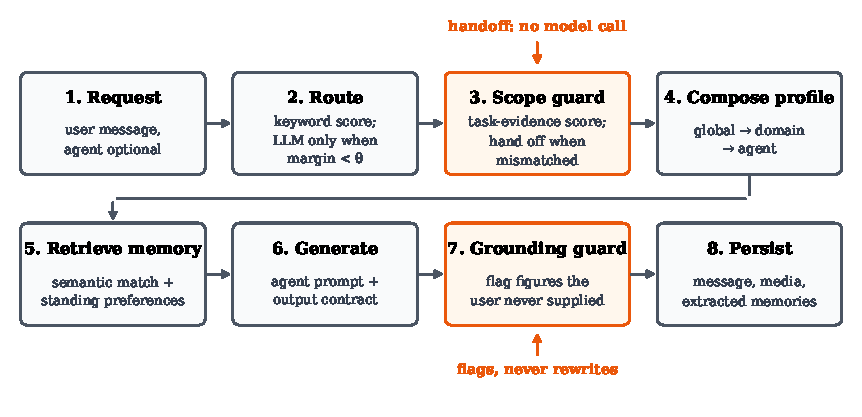
\includegraphics[width=0.96\textwidth]{fig1_pipeline.pdf}
\caption{The request pipeline. Stages 3 and 7 are deterministic: the scope
guard redirects a mismatched request with no model call, and the grounding
guard annotates unsupported figures without altering the generated text.}
\label{fig:pipeline}
\end{figure*}

\subsection{Three-Level Profile Composition}
A user holds a \textit{global} profile covering identity and communication
style, a \textit{domain} profile which for marketing carries brand name,
industry, audience, tone, palette and prohibited terms, and an \textit{agent}
profile which for the caption writer carries platforms, target length and
hashtag policy. At request time the three are composed into a context block,
with the narrowest scope taking precedence. A brand tone is stated once and
reaches all five agents; a hashtag policy reaches only the agent for which it
is meaningful.

\subsection{Deterministic Scope Guard}
Let $a$ be the selected agent and $S$ the set of sibling agents. For a request
$r$ we compute a task-evidence score $\tau(x, r)$ for each agent $x$,
accumulating matches of $r$ against the task vocabulary declared by $x$. The
request is redirected to $x^\star = \arg\max_{x \in S} \tau(x, r)$ when all of
the following hold:
\begin{align}
|r| &\ge \lambda_{\min} \label{eq:len}\\
\tau(a, r) &\le \theta_{\text{own}} \label{eq:own}\\
\tau(x^\star, r) &\ge \theta_{\text{other}} \label{eq:other}\\
\tau(x^\star, r) - \tau(a, r) &\ge \delta \label{eq:margin}
\end{align}
with $\lambda_{\min}=15$ characters, $\theta_{\text{own}}=1.5$,
$\theta_{\text{other}}=4.0$ and $\delta=3.0$. The thresholds are deliberately
conservative: a wrong redirect is more damaging to trust than a slightly
off-topic answer, so the guard stays silent unless the mismatch is clear.
Condition (\ref{eq:len}) suppresses the guard for greetings and
acknowledgements, which carry no task evidence either way. Condition
(\ref{eq:own}) requires that the selected agent be a genuinely poor fit rather
than merely a worse one, and conditions (\ref{eq:other}) and
(\ref{eq:margin}) require that some sibling be both strongly indicated and
clearly better. All four must hold, so a request that is ambiguous between two
agents is answered by the one the user chose.

One detail proved essential. An early version scored agents using their full
declared vocabulary, including their own \textit{names}. A request such as
``design an ad creative for the free trial'' sent to the caption writer then
scored highly for the caption writer, because the phrase contains words that
appear in its own name, and the request was never redirected. Restricting
$\tau$ to \textit{task} evidence and excluding name matches fixed this. The
router, which selects an agent when the user has not, continues to use the full
score, since there a name match is a legitimate signal of intent.

\subsection{Grounding Guard}
Let $P$ be a set of claim-shaped patterns: percentages, currency amounts, bare
multipliers such as tenfold, and ``up to'' constructions, declared per agent.
Let $N(r, \alpha, \pi)$ be the set of numeric tokens appearing in the request
$r$, any attachment $\alpha$, and the composed profile $\pi$. For generated
text $g$, every match $m \in P$ whose numeric token $n(m)$ does not belong to
$N(r,\alpha,\pi)$ is flagged. The reply is returned unchanged with an appended
notice naming the unsupported figures.

Three refinements were required by observed false positives.
\textit{Cadence expressions} such as ``three times per week'' are schedules,
not claims, and are excluded by a negative lookahead over temporal units.
\textit{Self-labelled proposals} such as a percentage annotated as a suggested
figure are explicitly marked as proposals, which is behavior the campaign
planner's instructions request, and flagging them penalized compliance.
\textit{Budget allocation} is legitimate for the planner: given a user-supplied
total $T$, currency amounts no greater than $T$ are permitted, enabled per
agent so the exemption does not leak to agents that have no business
allocating money.

The guard reads text only. When a user attaches an image, a figure the model
read off that image is indistinguishable from one it invented, so the notice
changes wording to say the check cannot see images rather than asserting
fabrication.

\section{Evaluation Methodology}

\subsection{Dataset}
The dataset is 30 request cases held as declarative data, spanning twelve
categories (\tabref{tab:dataset}). Categories were chosen to cover the failure
modes we cared about rather than to sample naturally occurring traffic, a
limitation we return to in Section 7. Five cases are marked as requiring a real
model and are skipped under the deterministic composer, because that composer
ignores agent instructions by construction and running them would say nothing
about prompt quality.

\begin{table}[t]
\centering
\caption{Composition of the Evaluation Dataset of 30 Request Cases}
\label{tab:dataset}
\small
\begin{tabular}{@{}lr@{\hspace{1.6em}}lr@{}}
\toprule
Category & $n$ & Category & $n$\\
\midrule
Ordinary        & 7 & Grounding      & 4\\
Out of scope    & 6 & Complex        & 3\\
Profile         & 2 & Routing        & 2\\
Ambiguous       & 1 & Attachment     & 1\\
Brand           & 1 & Clarification  & 1\\
Memory          & 1 & Platform       & 1\\
\bottomrule
\end{tabular}
\tabnote{Categories are disjoint. ``Out of scope'' and ``Routing'' cases
produce a handoff rather than creative output and are therefore excluded from
judge scoring.}
\end{table}

\subsection{Deterministic Assertions}
Each case declares machine-checkable assertions: expected output kind, whether
a scope handoff should occur and to which agent, rendered media dimensions,
substrings that must or must not appear, hashtag and length limits, whether
profile content reached the assembled prompt, and whether a stored memory was
retrieved. A run yields 110 assertions over the 30 cases. Every run records the
provider, model, temperature, token budget, embedding configuration and guard
thresholds, and the comparison tool refuses to compare runs that differ in
these respects.

\subsection{Rubric and Judge}
Qualitative dimensions are defined in a human-readable rubric of 32 dimensions
across five groups, each with anchors at levels 1, 3 and 5. A case declares
which dimensions apply to it; 22 of the 30 cases are scorable, the remaining
eight being scope handoffs and routing decisions that produce no creative
output.

The judge receives the brand context the run actually configured, the request,
the output, and the anchors for that case's dimensions, and returns a score and
a one-sentence justification per dimension at temperature zero. Two dimensions,
legibility and brand fit, are properties of rendered pixels; since the judge
receives only the image specification and alternative text, these are reported
as unjudged rather than guessed. Layout legibility is instead checked
deterministically across 27 size-and-payload combinations.

The rubric is parsed from the same prose document a human reader uses, so the
machine-readable and human-readable versions cannot diverge. A consistency
check asserts in both directions that every dimension a case declares exists in
the rubric and every dimension defined is used by some case.

\subsection{Reliability Protocol}
\label{sec:protocol}
The protocol below is what Subsection 5.2 quantifies, and what every comparison
in Subsection 5.4 depends on.

The judge scores each case $N$ times. We report the \textit{median} as the
score and the \textit{spread}, that is the maximum minus the minimum, as the
uncertainty. With $N=1$ no spread is reported, since unknown is not the same as
zero. Runs are comparable only when judge model, judge prompt version, rubric
file and $N$ all match, and the comparison tool enforces this. When the judge
model equals the model that produced the output, the condition is flagged in
the terminal, the stored results and the rendered report, because
self-preference makes such a figure an upper bound rather than a
measurement~\cite{panickssery2024selfpref}.

\subsection{Reproducibility}
All reported numbers derive from stored run artefacts rather than from
transcription: every figure in this paper is generated by a script that reads
those artefacts, so a figure cannot drift from the result it depicts. Hardware
was a four-core mobile processor without a graphics accelerator. Local models
ran under a self-hosted runtime; hosted models were reached through a
vendor-neutral chat-completions interface. The source code, dataset and all run
reports will be released publicly on acceptance; they are withheld during
review to preserve anonymity.

\section{Results}

\subsection{Effect of the Deterministic Guards}
\tabref{tab:rq1} reports the deterministic suite before and after the guards,
holding the model and all settings fixed at a local three-billion-parameter
model.

\begin{table}[t]
\centering
\caption{Deterministic Suite Before and After the Guards, With Model and
Settings Held Identical}
\label{tab:rq1}
\small
\begin{tabular}{@{}lcc@{}}
\toprule
 & Baseline & With guards\\
\midrule
Assertions passed             & 102/105 & \textbf{105/108}\\
Errors                        & 0 & 0\\
Degraded image specifications & 0 & 0\\
Routing of ``write ad copy''  & Image agent & \textbf{Caption agent}\\
Supplied budget of 400        & Not asserted & \textbf{Sums to 400}\\
Invented figures              & Undetected & \textbf{Flagged}\\
Elapsed, 21 generating cases  & 1215 s & 1322 s\\
\bottomrule
\end{tabular}
\tabnote{The guards add three assertions, which pass. Elapsed time rises by
9\%, which is the cost of longer instructions.}
\end{table}

Three failures persisted, all on cases requiring the model to ask a clarifying
question or to refrain from inventing figures. No prompt revision moved them.
Substituting a larger hosted model, with every other setting unchanged, closed
all three and reduced elapsed time from 1325 s to 88 s. We therefore attribute
those residual failures to model capability rather than system design, a
distinction that deterministic assertions alone cannot draw, and that only a
controlled model substitution could establish.

That substitution also exposed two false positives in our own grounding guard
that the weaker model had never triggered, because it never produced the
constructions involved: a posting cadence and a self-labelled proposal, both
described in Subsection 3.4. Both were corrected, and the corrected guard is
checked in both directions, so unlabelled claims are still caught.

\subsection{Judge Reliability and a Rubric-Induced Scale Collapse}

Judging the full suite with an independent model, not the generator, produced a
mean of 4.23 out of 5 across 61 dimension scores. Taken alone this number is
close to meaningless, which is the point of this subsection.

First, the scale. Across 174 individual judgements under our initial judge
prompt, \textit{every score was 1, 3 or 5}; levels 2 and 4 were never used
(\figref{fig:collapse}). The cause was the rubric: its tables define anchors at
1, 3 and 5, and the judge treated those as the only admissible answers. A
five-point instrument had silently become a three-point one. Naming the
intermediate levels explicitly in the prompt restored them, with 10.4\% of
subsequent scores even-valued, and reduced the worst observed spread from 4 to
2.

\begin{figure}[t]
\centering
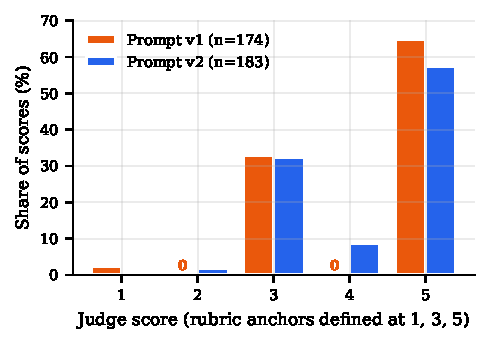
\includegraphics[width=\columnwidth]{fig2_scale_collapse.pdf}
\caption{Judge score distribution before and after the judge prompt named the
intermediate scale levels. Under version 1 no score of 2 or 4 occurred in 174
judgements, because the rubric defines anchors only at 1, 3 and 5.}
\label{fig:collapse}
\end{figure}

Second, the variance. Scoring identical outputs three times at temperature zero
gave 62\%--69\% exact agreement, a mean spread of 0.51--0.54 and a worst-case
spread of 4 on a five-point scale. Re-running an unchanged configuration and
re-judging moved one agent's mean by 0.37 with no change to the system at all.
We adopt 0.5 as the noise floor for this task: differences below it are not
results. An earlier screening pass used 0.33 and duly identified two per-agent
winners that Subsection 5.4 shows to be spurious.

Scores are therefore comparable only within a fixed judge model, prompt version
and repeat count, all of which we record with every stored result.

\subsection{How Much Does the Generator Model Matter?}

We evaluated every model available to us at no cost, seven of the twenty-two
offered by the hosted provider, the remainder requiring paid credits, holding
the dataset, thresholds and judge fixed and changing only the generator
(\tabref{tab:bakeoff}, \figref{fig:bakeoff}).

\begin{table}[t]
\centering
\caption{Seven-Model Comparison With Dataset, Thresholds and Judge Held Fixed}
\label{tab:bakeoff}
\small
% Models are named, not anonymised: identifiers do not reveal the authors, and
% naming them is required for the result to be checkable and for the table to
% agree with Fig.3.
\begin{tabular}{@{}lccrc@{}}
\toprule
Model & Judge & Assertions & Time (s) & Errors\\
\midrule
beam                 & 4.16 & 108/110 & 142 & 0\\
gemma4:31b           & 4.15 & 109/110 & \textbf{43} & 0\\
gpt-oss:20b          & 3.89 & 105/110 & 113 & 0\\
nemotron-3-ultra     & 3.87 & 107/110 & 386 & 0\\
nemotron-3-super     & 3.80 & 107/110 & 731 & 0\\
gpt-oss:120b         & 3.52 & 103/110 & 83  & 0\\
nemotron-3-nano:30b  & ---  & 80/82   & 563 & 9\\
\bottomrule
\end{tabular}
\tabnote{gpt-oss:120b judged its own output, so its score is an upper bound.
nemotron-3-nano:30b is excluded from the quality comparison: 9 of its 30 cases
errored, so its mean describes an easier subset.}
\end{table}

\begin{figure}[t]
\centering
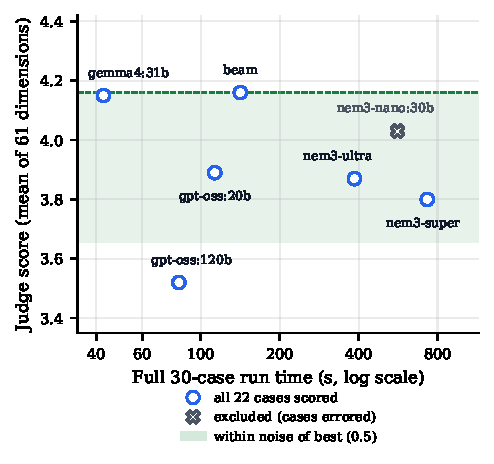
\includegraphics[width=\columnwidth]{fig3_bakeoff.pdf}
\caption{Judge score against wall-clock run time for every freely available
model. Five of six comparable models fall within the measured noise floor of
the best, while run time varies by a factor of seventeen.}
\label{fig:bakeoff}
\end{figure}

The leading two models differ by 0.01, far inside the noise floor, while
differing by a factor of 3.3 in run time. Five of the six comparable models lie
within 0.5 of the best. The practical conclusion is that for this task,
selection among freely available models should be driven by latency and
reliability, which are measured precisely, rather than by judge score, which is
not.

Two incidental findings deserve note. The largest model tested scored
\textit{lowest} despite judging its own output, a condition that should have
inflated it. And one model could not complete the suite at all, for a reason
that turned out to be a defect in our own client (Subsection 5.6).

\subsection{Per-Agent Model Specialization}

A multi-agent architecture invites the hypothesis that each specialized agent
should use the model best suited to it. The screening pass in Subsection 5.3
appeared to support this, identifying two agents whose scores improved by 0.45
and 0.33 under non-default models.

We tested the hypothesis directly. A mixed-fleet configuration pinned those two
agents to their apparent best models; a control arm used one model throughout.
Both arms were freshly generated and judged under the protocol of
Subsection 4.4 with three repeats (\figref{fig:ab}, \tabref{tab:ab}).

\begin{table}[t]
\centering
\caption{Paired Comparison of One Model Serving All Agents Against a Mixed
Fleet}
\label{tab:ab}
\small
\begin{tabular}{@{}lcc@{}}
\toprule
 & One model & Mixed fleet\\
\midrule
Overall judge mean       & \textbf{4.28} & 4.18\\
Assertions               & 109/110 & 109/110\\
Elapsed                  & \textbf{54 s} & 201 s\\
Advertisement agent      & \textbf{4.56} & 4.33\\
Caption agent            & 3.80 & \textbf{3.87}\\
Post-image agent         & \textbf{4.25} & 3.88\\
\bottomrule
\end{tabular}
\tabnote{The advertisement and caption agents are the two that were pinned to
non-default models. The post-image agent used the same model in both arms, and
its mean nonetheless moved by 0.37.}
\end{table}

\begin{figure}[t]
\centering
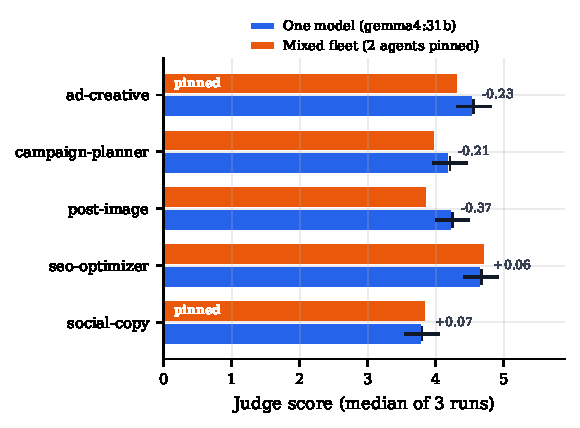
\includegraphics[width=\columnwidth]{fig4_ab_per_agent.pdf}
\caption{Per-agent scores for both arms. Whiskers show the judge's own mean
spread on the control arm. Every between-arm gap, including for the two pinned
agents, lies inside that spread.}
\label{fig:ab}
\end{figure}

Of 61 paired dimension scores, 46 were unchanged. Among the 15 that moved, 7
favoured the mixed fleet and 8 the single model. A Wilcoxon signed-rank
test~\cite{wilcoxon1945} on the paired scores gives $W = 45.5$ with $n = 15$
and $p = 0.42$, exact and two-sided, with an effect size of $d = -0.12$: no
significant difference and a negligible effect. We use a signed-rank test
rather than a paired $t$-test because the scores are ordinal and discrete, and
the exact distribution is tractable at this sample size. The mixed fleet was
nonetheless 3.7 times slower.

The decisive observation is the last row of \tabref{tab:ab}. The post-image
agent used the \textit{same} model in both arms and its mean still moved by
0.37. Generation at non-zero temperature plus judge disagreement produces
per-agent movement of that magnitude with no configuration change whatsoever.
The screening gaps of 0.33 and 0.45 were within that band, and did not survive
confirmation; one of the two pinned agents became measurably worse.

We therefore reject the per-agent specialization hypothesis at this scale. We
emphasise that this is a negative result about effect size relative to noise,
not evidence that model choice never matters; a task with wider genuine quality
separation could well reach the opposite conclusion.

\subsection{Self-Audit: Defects in the Evaluation Apparatus}

Two defects in the evaluation were found by running it, and both would have
silently corrupted conclusions.

The scale collapse of Subsection 5.2 is the first. A rubric that reads
correctly to a human restricted the judge to three of five levels across 174
judgements. Nothing in the pipeline would have surfaced this; it was visible
only on inspecting the score distribution, which we had no particular reason to
plot.

The second was a self-contradictory test case. A case intended to test profile
awareness configured the agent's content type as a landing page while the
request asked for a blog post. The agent followed the explicit request and
stated that it had done so, which is the correct precedence. The rubric anchor
for that dimension rewarded adherence to the configured profile, and so scored
correct behavior 1 out of 5, unanimously across three repeats. The defect lay
in the rubric and the case, not the system. We corrected the anchor to state
that an explicit request overrides a standing default, removed the
contradiction from the case, and added a companion case that deliberately
exercises the override.

Both incidents share a shape: the apparatus was internally consistent and
externally wrong, and the error presented as a confident number.

\subsection{A Client Defect Presenting as Provider Failure}

During the model comparison, four of six models failed between 4 and 19 of 30
cases with what appeared to be provider outages. The cause was neither the
provider nor the models. Models that spend completion tokens on hidden
reasoning before answering can exhaust the token budget mid-thought, in which
case the interface returns a success status with an empty message body and a
finish reason of length. Our client treated an empty body as a provider
failure. On one model, one request in six returned 700 completion tokens and
zero characters of content.

Treating that specific signature, namely empty content with a length finish
reason or a populated reasoning field with no answer, as a budget condition and
retrying once with threefold headroom reduced five of six models to zero
errors. The sixth remains unusable for this task: it produced 12\,000 to
16\,000 characters of reasoning and no answer even at a 4000-token ceiling,
requiring 41 retries in a single run.

We report this because it affected comparability rather than merely robustness.
Before the fix, each model errored on a different number of cases, so each
model's score described a different subset of the dataset. Any ranking computed
across those runs would have been an artefact of which cases happened to
survive.

\subsection{Latency and Cost}
\tabref{tab:perf} contrasts a local three-billion-parameter model on commodity
hardware with a hosted thirty-one-billion-parameter model. On a processor
without a graphics accelerator, prompt evaluation dominates, so latency tracks
prompt size as much as reply length.

\begin{table}[t]
\centering
\caption{Latency and Cost on a Four-Core Mobile Processor Without a Graphics
Accelerator}
\label{tab:perf}
\small
\begin{tabular}{@{}lcc@{}}
\toprule
Operation & Local model & Hosted model\\
\midrule
Text agent                     & 28--53 s & 1.3--3.2 s\\
Image agent, spec and render   & 28--64 s & 1.4--2.4 s\\
Scope handoff                  & $<$1 ms & $<$1 ms\\
Full 30-case run               & 1325 s & 49--88 s\\
Cost per run                   & ---     & 0.0039 USD\\
\bottomrule
\end{tabular}
\tabnote{The scope handoff requires no model call, so a redirected request
costs no tokens and returns effectively instantly regardless of backend.}
\end{table}

\section{Discussion}

\textbf{Prompt instructions are not a safety mechanism.} Explicit prohibition
did not stop figure fabrication; a deterministic post-processing check did. This
agrees with the premise behind programmable guardrail
systems~\cite{rebedea2023nemo} and suggests a simple design heuristic: if a
property can be checked in code, check it in code, and reserve the model for
what only a model can do.

\textbf{Flagging beats rewriting for provenance.} An automatic rewrite that
removes an unsupported figure damages the sentence containing it, and the system
cannot know whether the claim was true, since only the user can. Annotating
preserves both the text and the user's authority over it.

\textbf{Report the noise floor, not just the score.} This is our main
methodological claim. Our judge disagreed with itself by roughly half a point
on a five-point scale, and total run-to-run movement reached 0.37 on an
unchanged configuration. Differences of 0.3 are routinely presented as
improvements in informal practice. Publishing a judge score without its
variance invites exactly the error we made during screening and caught only by
confirming. A noise floor is cheap to obtain, requiring only that the judge be
run $N$ times and the spread reported, and it changes which conclusions are
available.

\textbf{Architectural specialization does not imply model specialization.} The
appeal of giving each narrow agent its own model is strong and, at this scale,
unsupported: no significant difference, a negligible effect size, 3.7 times the
latency and more operational complexity. One model served five agents as well
as five models did.

\textbf{Evaluation code deserves the same scrutiny as system code.} Both
defects in Subsection 5.5 were in the measuring apparatus, and both produced
plausible numbers. We found them only because we plotted a distribution and
re-read a low score we did not believe.

\subsection{Implications for Practitioners}
Four findings translate directly into deployment practice, and we state them
separately because each is cheap to adopt.

First, separate the two kinds of check. Deterministic assertions over
machine-verifiable properties are fast, free and stable, and they should carry
as much of the evaluation burden as possible; reserve judge scoring for
properties that genuinely require reading. In our suite, 110 assertions cover
routing, handoff, provenance, geometry, length and profile propagation, leaving
32 rubric dimensions for the judge.

Second, record the configuration with the result. Every stored run in this work
carries its provider, model, temperature, token budget, embedding settings,
guard thresholds and, after the defect in Subsection 5.6, its per-agent model
assignments. The comparison tool refuses to compare runs that differ in any of
these. This sounds bureaucratic until a mixed-model run is indistinguishable
from a single-model run in the archive, which was briefly the case here.

Third, make the evaluator's uncertainty a first-class output. Reporting a
median with its spread costs one extra field and $N$ times the judge calls, in
our case 213 s and no monetary cost, and it is the difference between a
conclusion and a guess.

Fourth, prefer flagging to silent correction wherever the system cannot verify
the property itself. The grounding guard annotates, the scope guard redirects
and says why, and the empty-reply handler retries and then reports the specific
cause. In each case the user retains the information needed to override the
system, which matters more in content generation than a marginally cleaner
output would.

\section{Threats to Validity}

\textbf{Construct validity.} Judge scores are a proxy for human judgement, not
a measurement of quality. We did not conduct a human scoring pass, so we cannot
report agreement between our judge and human raters; this is the most important
limitation of the work. Self-preference was controlled by using a judge
different from the generator in all reported comparisons and by flagging the
one case where it was not, but verbosity and leniency effects were not
controlled: 36 of 61 median scores were 5s.

\textbf{Internal validity.} Agents generate at a temperature of 0.4, so arms
differ in generated text as well as configuration; our paired comparison
therefore measures the combined effect, and we report the control arm's own
variance to bound it. The signed-rank test rests on 15 non-tied pairs, which is
small, and a larger dataset could detect effects we cannot. Two of the scored
dimensions were excluded as unjudgeable from text, so image agents are scored
on fewer dimensions than text agents.

\textbf{External validity.} All results use a single synthetic brand in one
industry, one language and one set of five agents. The 30 cases were authored
to probe failure modes we anticipated, not sampled from production traffic, so
category proportions do not reflect real usage. The free-model set is specific
to one provider at one point in time, and model availability changes. The noise
floor of 0.5 is a property of this task and judge, not a constant.

\textbf{Conclusion validity.} Our fourth research question reports a negative
result; absence of a significant difference at this sample size is not evidence
of absence of any effect. Our claim is bounded accordingly: per-agent
specialization is unjustified \textit{at this scale and for this task}, because
any true effect is smaller than the variance we measured.

\section{Conclusions}

We presented a personalized multi-agent content generation system in which
scope enforcement and claim grounding are deterministic rather than
prompt-mediated, and a measurement study of what can honestly be concluded
about such a system. The guards took the deterministic suite from 102 of 105
assertions to 110 of 110 once a capable model was used, and a controlled model
substitution showed the residual failures to be a capability limit rather than
a design defect.

The measurement results are the more transferable contribution. An automatic
judge applied to this task disagreed with itself by a mean spread of 0.51--0.54
on a five-point scale, and an unchanged configuration moved a per-agent mean by
0.37. Against that floor, neither the seven-model comparison nor a paired
comparison of per-agent model assignment showed a significant benefit, and the
mixed fleet cost 3.7 times the latency. Running the evaluation also surfaced
two defects in the evaluation itself, each of which had been producing
confident and wrong numbers.

We conclude that judge-derived comparisons should be published with a measured
noise floor, that evaluation apparatus warrants the same testing discipline as
the system under test, and that architectural specialization should not be
assumed to justify model specialization without a paired, repeated measurement.

Future work should establish agreement between automatic and human judgement
for this task, extend the dataset beyond a single brand and language, and test
whether the noise floor we measured is characteristic of marketing-copy
evaluation or of our judge in particular.

\balance

\begin{thebibliography}{99}
\footnotesize

\bibitem{ji2023hallucination}
Ji Z, Lee N, Frieske R, Yu T, Su D, Xu Y, Ishii E, Bang Y, Madotto A, Fung P.
Survey of hallucination in natural language generation. \textit{ACM Computing
Surveys}, 2023, 55(12): 1--38.

\bibitem{wu2023autogen}
Wu Q, Bansal G, Zhang J, Wu Y, Li B, Zhu E, Jiang L, Zhang X, Zhang S, Liu J,
Awadallah A H, White R W, Burger D, Wang C. AutoGen: Enabling next-generation
large language model applications via multi-agent conversation. arXiv:2308.08155,
2023.

\bibitem{langgraph2024}
LangChain. LangGraph: Build resilient language agents as graphs. Technical
documentation, 2024.

\bibitem{rebedea2023nemo}
Rebedea T, Dinu R, Sreedhar M, Parisien C, Cohen J. NeMo Guardrails: A toolkit
for controllable and safe large language model applications with programmable
rails. In \textit{Proc. the 2023 Conference on Empirical Methods in Natural
Language Processing: System Demonstrations}, Dec. 2023, pp.431--445.

\bibitem{zheng2023judging}
Zheng L, Chiang W L, Sheng Y, Zhuang S, Wu Z, Zhuang Y, Lin Z, Li Z, Li D,
Xing E P, Zhang H, Gonzalez J E, Stoica I. Judging large language models as
judges with MT-Bench and Chatbot Arena. In \textit{Advances in Neural
Information Processing Systems 36}, Dec. 2023.

\bibitem{liu2023geval}
Liu Y, Iter D, Xu Y, Wang S, Xu R, Zhu C. G-Eval: Natural language generation
evaluation using large language models with better human alignment. In
\textit{Proc. the 2023 Conference on Empirical Methods in Natural Language
Processing}, Dec. 2023, pp.2511--2522.

\bibitem{panickssery2024selfpref}
Panickssery A, Bowman S R, Feng S. Large language model evaluators recognize
and favor their own generations. arXiv:2404.13076, 2024.

\bibitem{wang2023fair}
Wang P, Li L, Chen L, Cai Z, Zhu D, Lin B, Cao Y, Liu Q, Liu T, Sui Z. Large
language models are not fair evaluators. arXiv:2305.17926, 2023.

\bibitem{koo2023benchmarking}
Koo R, Lee M, Raheja V, Park J I, Kim Z M, Kang D. Benchmarking cognitive
biases in large language models as evaluators. arXiv:2309.17012, 2023.

\bibitem{koren2009matrix}
Koren Y, Bell R, Volinsky C. Matrix factorization techniques for recommender
systems. \textit{Computer}, 2009, 42(8): 30--37.

\bibitem{zhang2020explainable}
Zhang Y, Chen X. Explainable recommendation: A survey and new perspectives.
\textit{Foundations and Trends in Information Retrieval}, 2020, 14(1): 1--101.

\bibitem{lewis2020rag}
Lewis P, Perez E, Piktus A, Petroni F, Karpukhin V, Goyal N, K\"uttler H, Lewis
M, Yih W T, Rockt\"aschel T, Riedel S, Kiela D. Retrieval-augmented generation
for knowledge-intensive natural language processing tasks. In \textit{Advances
in Neural Information Processing Systems 33}, Dec. 2020, pp.9459--9474.

\bibitem{salemi2023lamp}
Salemi A, Mysore S, Bendersky M, Zamani H. LaMP: When large language models
meet personalization. arXiv:2304.11406, 2023.

\bibitem{brown2020fewshot}
Brown T B, Mann B, Ryder N, Subbiah M, Kaplan J, Dhariwal P, Neelakantan A,
Shyam P, Sastry G, Askell A \textit{et al}. Language models are few-shot
learners. In \textit{Advances in Neural Information Processing Systems 33},
Dec. 2020, pp.1877--1901.

% Order follows first citation in the text, per JCST 3.2.2: CrewAI is cited
% in Subsection 2.2 ahead of the transformer reference.
\bibitem{moura2024crewai}
Moura J. CrewAI: Framework for orchestrating role-playing autonomous agents.
Software repository, 2024.

\bibitem{vaswani2017attention}
Vaswani A, Shazeer N, Parmar N, Uszkoreit J, Jones L, Gomez A N, Kaiser L,
Polosukhin I. Attention is all you need. In \textit{Advances in Neural
Information Processing Systems 30}, Dec. 2017, pp.5998--6008.

\bibitem{yao2023react}
Yao S, Zhao J, Yu D, Du N, Shafran I, Narasimhan K, Cao Y. ReAct: Synergizing
reasoning and acting in language models. In \textit{Proc. the 11th
International Conference on Learning Representations}, May 2023.

\bibitem{wei2022cot}
Wei J, Wang X, Schuurmans D, Bosma M, Ichter B, Xia F, Chi E, Le Q, Zhou D.
Chain-of-thought prompting elicits reasoning in large language models. In
\textit{Advances in Neural Information Processing Systems 35}, Dec. 2022,
pp.24824--24837.

\bibitem{schick2023toolformer}
Schick T, Dwivedi-Yu J, Dess\`i R, Raileanu R, Lomeli M, Hambro E, Zettlemoyer
L, Cancedda N, Scialom T. Toolformer: Language models can teach themselves to
use tools. In \textit{Advances in Neural Information Processing Systems 36},
Dec. 2023.

\bibitem{shinn2023reflexion}
Shinn N, Cassano F, Gopinath A, Narasimhan K, Yao S. Reflexion: Language agents
with verbal reinforcement learning. In \textit{Advances in Neural Information
Processing Systems 36}, Dec. 2023.

\bibitem{manakul2023selfcheckgpt}
Manakul P, Liusie A, Gales M J F. SelfCheckGPT: Zero-resource black-box
hallucination detection for generative large language models. In \textit{Proc.
the 2023 Conference on Empirical Methods in Natural Language Processing},
Dec. 2023, pp.9004--9017.

\bibitem{min2023factscore}
Min S, Krishna K, Lyu X, Lewis M, Yih W T, Koh P W, Iyyer M, Zettlemoyer L,
Hajishirzi H. FActScore: Fine-grained atomic evaluation of factual precision in
long form text generation. In \textit{Proc. the 2023 Conference on Empirical
Methods in Natural Language Processing}, Dec. 2023, pp.12076--12100.

\bibitem{es2024ragas}
Es S, James J, Espinosa-Anke L, Schockaert S. RAGAS: Automated evaluation of
retrieval augmented generation. In \textit{Proc. the 18th Conference of the
European Chapter of the Association for Computational Linguistics: System
Demonstrations}, Mar. 2024, pp.150--158.

\bibitem{chiang2024arena}
Chiang W L, Zheng L, Sheng Y, Angelopoulos A N, Li T, Li D, Zhang H, Zhu B,
Jordan M, Gonzalez J E, Stoica I. Chatbot Arena: An open platform for
evaluating large language models by human preference. In \textit{Proc. the 41st
International Conference on Machine Learning}, Jul. 2024.

\bibitem{wang2023selfconsistency}
Wang X, Wei J, Schuurmans D, Le Q, Chi E, Narang S, Chowdhery A, Zhou D.
Self-consistency improves chain of thought reasoning in language models. In
\textit{Proc. the 11th International Conference on Learning Representations},
May 2023.

\bibitem{wilcoxon1945}
Wilcoxon F. Individual comparisons by ranking methods. \textit{Biometrics
Bulletin}, 1945, 1(6): 80--83.
\end{thebibliography}

% =============================== BODY-END ===========================
% JCST requires author biographies and 600 dpi photographs only upon
% acceptance, so none appear here.  On acceptance, add for each author:
%     \REPLACE{short biography and a 600 dpi photograph}

\end{document}
